%% ----------------------------------------------------------------
%% Article.tex
%% ---------------------------------------------------------------- 
\documentclass{ecsarticle}     % Use the Article Style
\graphicspath{{Figures/}}   % Location of your graphics files
\usepackage{natbib}            % Use Natbib style for the refs.
\hypersetup{colorlinks=false}   % Set to false for black/white printing
\input{Definitions}            % Include your abbreviations

\usepackage[nodayofweek]{datetime}
\usepackage{listings}
\usepackage{color}

\usepackage{graphicx}



%% ----------------------------------------------------------------
\begin{document}
%TC:ignore
\frontmatter
\title      {COMP6036: Advanced Machine Learning\\
            Feature Selection Challenge}
      
\addresses  {\deptname\\\univname}
\authors                 {\href{mailto:ajr2g10@ecs.soton.ac.uk}{Ashley J. Robinson}\\\href{mailto:ajr2g10@ecs.soton.ac.uk}{ajr2g10@ecs.soton.ac.uk}}

\date       {\today}
\subject    {}
\keywords   {}
\maketitle
%% ----------------------------------------------------------------


\begin{abstract}
\end{abstract}

%TC:endignore
\mainmatter


\section{Introduction}

Each dataset has been divided in three section for training, validation and test submission.
The final partition labels remain hidden from the development process.
The discrete class labels, $t$, and the classifier outputs, $y$, are described by equation~\eqref{eqn:output}.
Keeping to these output values requires using the thresholding function $\Theta$ in equation~\eqref{eqn:theta}. 
Everything implemented has been developed from scratch for the MATLAB programming language. 


\begin{equation}
	y,t \in \{-1,+1\}
	\label{eqn:output}
\end{equation}

\begin{equation}
	\Theta(a) = \left\{ 
      \begin{array}{l}
         +1,\:a > 0\\
         -1,\:a \leq 0\\
      \end{array} \right.	
	\label{eqn:theta}
\end{equation}

\section{Classifier Architectures}

Artificial Neural Networks (ANNs) have been chosen as the classifier architectures.
ANNs are efficient learning machines with biological inspiration~\citep{bishop06pattern}. 
They are parametric models which can be adapted during supervised training and are scalable in complexity.
The error space can be considered as a function of parameters and the training data, $E(w|D)$, therefore many different optimisation algorithms can be used can used to train the model. 



\subsection{Perceptron}
\label{sec:perceptron}

Figure~\ref{fig:slp} holds the most simple manifestation of an ANN called a perceptron.
Each feature of an input pattern is weighted and then summed, along with a bias term, to produce an output.
This output passes through a step activation function for binary classification.
Capable of producing a linear separation boundary subject to equation~\eqref{eqn:slp} the method serves as starting point for further investigation into the data.
The discrete error from from the training patterns is calculated using equation~\eqref{eqn:slp_error}.
Equation~\eqref{eqn:slp_mat} expands the method by considering many different training patterns applied to only one set of weights.
The weight vector is trained using the iterative learning rule held in equations~\eqref{eqn:slp_learn_1},~\eqref{eqn:slp_learn_2} and~\eqref{eqn:slp_learn_3}~\citep{info05mackay}.
In practice the offset parameter, $b$, is added to the weight vector and every input pattern is appended with a constant unit feature to allow complete training.

\begin{figure}[ht]
   \centering
    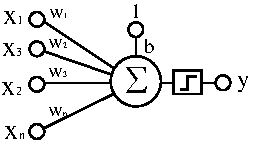
\includegraphics[width = 8cm]{SLP.pdf}
   \caption{Perceptron architecture.}
   \label{fig:slp}
\end{figure}

\begin{equation}
   y = \Theta \left(b + \sum_{i=1}^{n} w_i x_i \right)
   \label{eqn:slp}
\end{equation}

\begin{equation}	
	e = t - y,\:\:e \in \{-2,0.+2\}
	\label{eqn:slp_error}
\end{equation}

\begin{equation}
   \textbf{Y} = \Theta ( \textbf{X}.\textbf{W} + \textbf{b})
   \label{eqn:slp_mat}
\end{equation}

\begin{equation}	
	\textbf{W}_{t+1} = \textbf{W}_t + \Delta \textbf{W}
	\label{eqn:slp_learn_1}
\end{equation}

\begin{equation}	
	\mathbf{E} = (\mathbf{T} - \mathbf{Y})^{T}
	\label{eqn:slp_learn_2}
\end{equation}

\begin{equation}	
	\Delta \mathbf{W} = \mathbf{\eta}*\mathbf{E}\mathbf{X}^T
	\label{eqn:slp_learn_3}
\end{equation}


\subsection{Multi Layer Perceptron}
Section~\ref{sec:perceptron} can be expanded by concatenating the architecture to produce a multi layer perceptron.
They contain hidden layers and when used with non-linear activation functions can produced a non-linear separation boundary~\citep{bennett01ml}.
Only one hidden layer is implemented for simplicity as shown in Figure~\ref{fig:mlp}. 


\begin{figure}[ht]
   \centering
    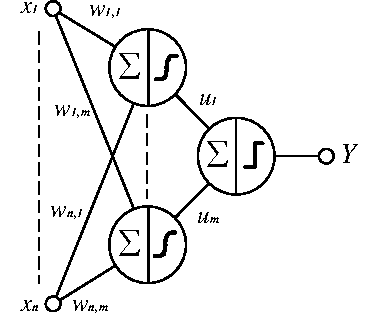
\includegraphics[width = 8cm]{MLP.pdf}
   \caption{Multi layer perceptron architecture.}
   \label{fig:mlp}
\end{figure}

\begin{equation}
   y = \Theta \left(b + \sum_{i=1}^{n} w_i x_i \right)
   \label{eqn:slp}
\end{equation}

\begin{equation}	
	e = t - y,\:\:e \in \{-2,0.+2\}
	\label{eqn:slp_error}
\end{equation}

\begin{equation}
   \textbf{Y} = \Theta ( \textbf{X}.\textbf{W} + \textbf{b})
   \label{eqn:slp_mat}
\end{equation}

\begin{equation}	
	\textbf{W}_{t+1} = \textbf{W}_t + \Delta \textbf{W}
	\label{eqn:slp_learn_1}
\end{equation}

\begin{equation}	
	\mathbf{E} = (\mathbf{T} - \mathbf{Y})^{T}
	\label{eqn:slp_learn_2}
\end{equation}

\begin{equation}	
	\Delta \mathbf{W} = \mathbf{\eta}*\mathbf{E}\mathbf{X}^T
	\label{eqn:slp_learn_3}
\end{equation}



\section{Feature Selection}

\section{Results}

\section{Conclusions}


\newpage

%TC:ignore
\bibliographystyle{ecs}
\bibliography{references}



\backmatter
\begin{appendix}

\newpage
\section{Code Listings}

\end{appendix}

%TC:endignore
\end{document}
%% ----------------------------------------------------------------

